\pagebreak
\section{Mobile UHF-Band MU-MIMO Channel Characterization}
\label{sec:uhf_mobile}

	In this final series of experiments, we wish to extend our investigation of \ac{MU-MIMO} beamforming to the case where \acp{STA} are mobile, both in indoor and outdoor environments.
	Intuitively, one can imagine that a beamforming \ac{AP} will have to continually steer the beam towards an intended user as the user moves, disrupting the temporal stability in \ac{TVWS} environments that we observed in the previous sections.
	While 802.11n/ac/af beamforming standards utilize channel sounding techniques that refresh the \ac{CSI} before each multi-user transmission, we are interested in leveraging UHF-band \ac{CSI} stability to re-use old or ``stale'' \ac{CSI} estimates.
	In this section, we explore the temporal characteristics of pedestrian mobile nodes and explore the timescales under which stale \ac{CSI} remains useful in real scenarios.

% Describe the S-T interval
\subsection{Sounding-Transmission (S-T) Interval}
\label{sec_st_interval}

	In the following analysis of various alternative resounding policies for 802.11af systems, we focus our analysis on the effect of the time interval between when a channel is sounded and when the final beamformed transmission takes place.
	We call this time the ``Sounding-Transmission Interval,'' or S-T interval.
	Differences in the sounded \ac{CSIT} compared to the actual physical channel at the time of zero-forcing transmission result in inter-stream interference between \acp{STA} as well as reduction in their desired signal strength.
	In mobile environments, it is highly likely that a larger S-T interval will yield higher inter-stream interference due to increased \ac{CSIT} error and therefore lower \ac{SINR}.
	
	%This staleness threshold is determined by the scenario and the target performance of the system. \csnote{this sounds really handwavy... either define the threshold here or point to where it is defined}

	The S-T interval is important for understanding the performance of opportunistic implicit sounding since an opportunistic \ac{AP} may have cached, or ``stale'' \ac{CSIT} obtained from previous uplink transmissions made at different times.
	In order to use this \ac{CSIT}, it will need to make a decision about future beamformed transmissions utilizing that stale \ac{CSIT}.
	On the other hand, an implicit or explicit \ac{AP} refreshes all \ac{CSIT} simultaneously at the beginning of a multi-user packet, yielding an S-T interval of nearly zero.
	
	Depending on the length of the S-T interval, an opportunistic system could exhibit high inefficiency due to unnecessary sounding overhead, or poor performance due to stale \ac{CSIT}.
	In order to emulate opportunistic collection of \ac{CSIT}, we need to characterize how drift in the \ac{CSI} of a single \ac{STA} will affect the performance of a future beamformed transmission including multiple other \acp{STA}.

%% Measurement Technique
\subsection{Experimental Setup}
\label{sec_uhf_mobile_setup}

	For mobility experiments, we wished to explore two scenarios: indoor with rich multipath in the same environment characterized in Section~\ref{sec_static_indoor_exp}; and outdoor with \ac{NLoS} coverage through dense trees.
	The locations for the indoor measurements performed in Rice University's Duncan Hall office building are given in Figure~\ref{fig_mobile_indoor_location}, with the mobile node labeled in black.
	The location for the outdoor measurement is shown in Figure~\ref{fig_mobile_outdoor_location}, where we moved outside the Houston City UHF protection contours in order to avoid evironmental noise and interference.

	We obtained experimental radio licenses from the \ac{FCC} with call signs WH2XJV and WJ9XFF to operate our experimental equipment on UHF channels and performed a series of indoor and outdoor measurement campaigns in various mobility scenarios to analyze \ac{MU-MIMO} beamforming capacity with respect to \ac{CSIT} overhead.

	%We leveraged our shift to the Argos architecture by porting the Argos synchronization and measurement framework first developed at Rice University to operate on Skylark's \ac{WURC} \ac{SDR} hardware.
	%This allowed us to quickly perform array calibration as well as provide a framework for node synchronization and fine-grained implicit channel measurements compared to in-house existing frameworks.
	We deployed the 8x8 \ac{TVWS} \ac{MU-MIMO} platform from Section~\ref{sec:wurc_argos_design} using the Argos mobile channel sounding framework as presented in Section~\ref{sec_mobile_chan_est} to increase the \ac{CSI} sampling resolution as well as to handle node synchronization over-the-air.
	Increased sampling resolution allowed us to track the mobile channel dynamics in ways that were not possible with WARPLab-based channel sounding due to WARPLab's processing latecy (Section~\ref{sec_warplab_timing}).
	
	The Argos channel sounding framework requires a side channel for command and control messaging, but since timing synchronization was handled over-the-air in-band, we could meet this requirement with a wireless 802.11n overlay wireless network operating at 5.8~GHz to avoid interference with our measurements.
	This timing synchronization allow us to have truly mobile, battery-powered \acp{STA}, since a low-latency ethernet backhaul was no longer needed.

	We used a linear antenna array of omnidirectional 3 dBi August DTA240 antennas separated by over a half-wavelength at the operational frequency of 629 MHz (Figure \ref{fig_array_truck}).

	%An Argos-WURC node consists of three components: 1) a WARPv3 \ac{SDR} kit from Mango Communications; 2) a Skylark 1x1 or 1x4 WAB adaptor board; 3) one or more Skylark \ac{WURC} front-ends.
	%Figure~\ref{fig_mobile_outdoor_ap} shows two 4x Argos-WURC base station nodes and 9 additional 1x Argos-WURC ``mobile'' nodes, with the omni-direction 3 dBi August DTA240 antennas used for the indoor measurements visible in the bottom left. Not all nodes were functional or available for all experiments.

	Figure~\ref{fig_array_truck} shows the hardware platform and linear antenna array with both properly-spaced UHF omni-directional antennas (black) and 2.4~GHz directional antennas (white) for comparison.
	Installed hanging from a tree in Figure~\ref{fig_array_tree}, we tried to best emulate an elevated \ac{AP} serving a population of fixed endpoint through a dense forest environment.
	Examples of the fixed \acp{STA} are shown in Figure~\ref{fig_sta_outdoor_tripod} for the outdoor nodes with battery-powered operation, while the indoor fixed nodes were deployed as shown in Figure~\ref{fig_sta_indoor_table} with a wired ethernet backhaul and AC power.
	In our outdoor measurements, performance of the 2.4~GHz band through dense vegetation was poor and spotty at best, so we omit those results.

%\begin{figure}[t] % WURCLab SISO Node
%\centering
%\includegraphics[width=1\linewidth]{./figs/platform_amalgam}
%\caption{Single-radio mobile node, omnidirectional antenna and outdoor installed \ac{AP}.}
%\label{fig_mobile_outdoor_ap}
%\end{figure}

% Indoor and Outdoor Measurement Locations
\begin{figure}[ht!]
\centering
\begin{minipage}{0.49\textwidth}
\centering
\includegraphics[width=1.0\linewidth]{figs/meas/duncan_layout}
\caption{Indoor node locations in Rice University Duncan Hall.}
\label{fig_mobile_indoor_location}
\end{minipage}
\hfill
\begin{minipage}{0.49\textwidth}
\centering
\includegraphics[width=1.0\linewidth]{figs/meas/protection_contours_trim}
\caption{Outdoor experiment location and \ac{TVWS} protection contours.}
\label{fig_mobile_outdoor_location}
\end{minipage}
\end{figure}

% Outdoor Measurement Platform
\begin{figure}[p]
\centering
\begin{minipage}{0.67\textwidth}
\centering
\includegraphics[width=1.0\linewidth]{figs/meas/array_on_truck}
\caption{8x8 \ac{AP} with linear antenna array.}
\label{fig_array_truck}
\end{minipage}
\hfill
\begin{minipage}{0.315\textwidth}
\centering
\includegraphics[width=1.0\linewidth]{figs/meas/array_on_tree}
\caption{8x8 \ac{AP} on tree.}
\label{fig_array_tree}
\end{minipage}
\end{figure}

% STA Measurement Platform
\begin{figure}[p]
\centering
\begin{minipage}{0.45\textwidth}
\centering
\includegraphics[width=1.0\linewidth]{figs/meas/example_single_node}
\caption{Static \ac{STA} for indoor tests.}
\label{fig_sta_indoor_table}
\end{minipage}
\hfill
\begin{minipage}{0.45\textwidth}
\centering
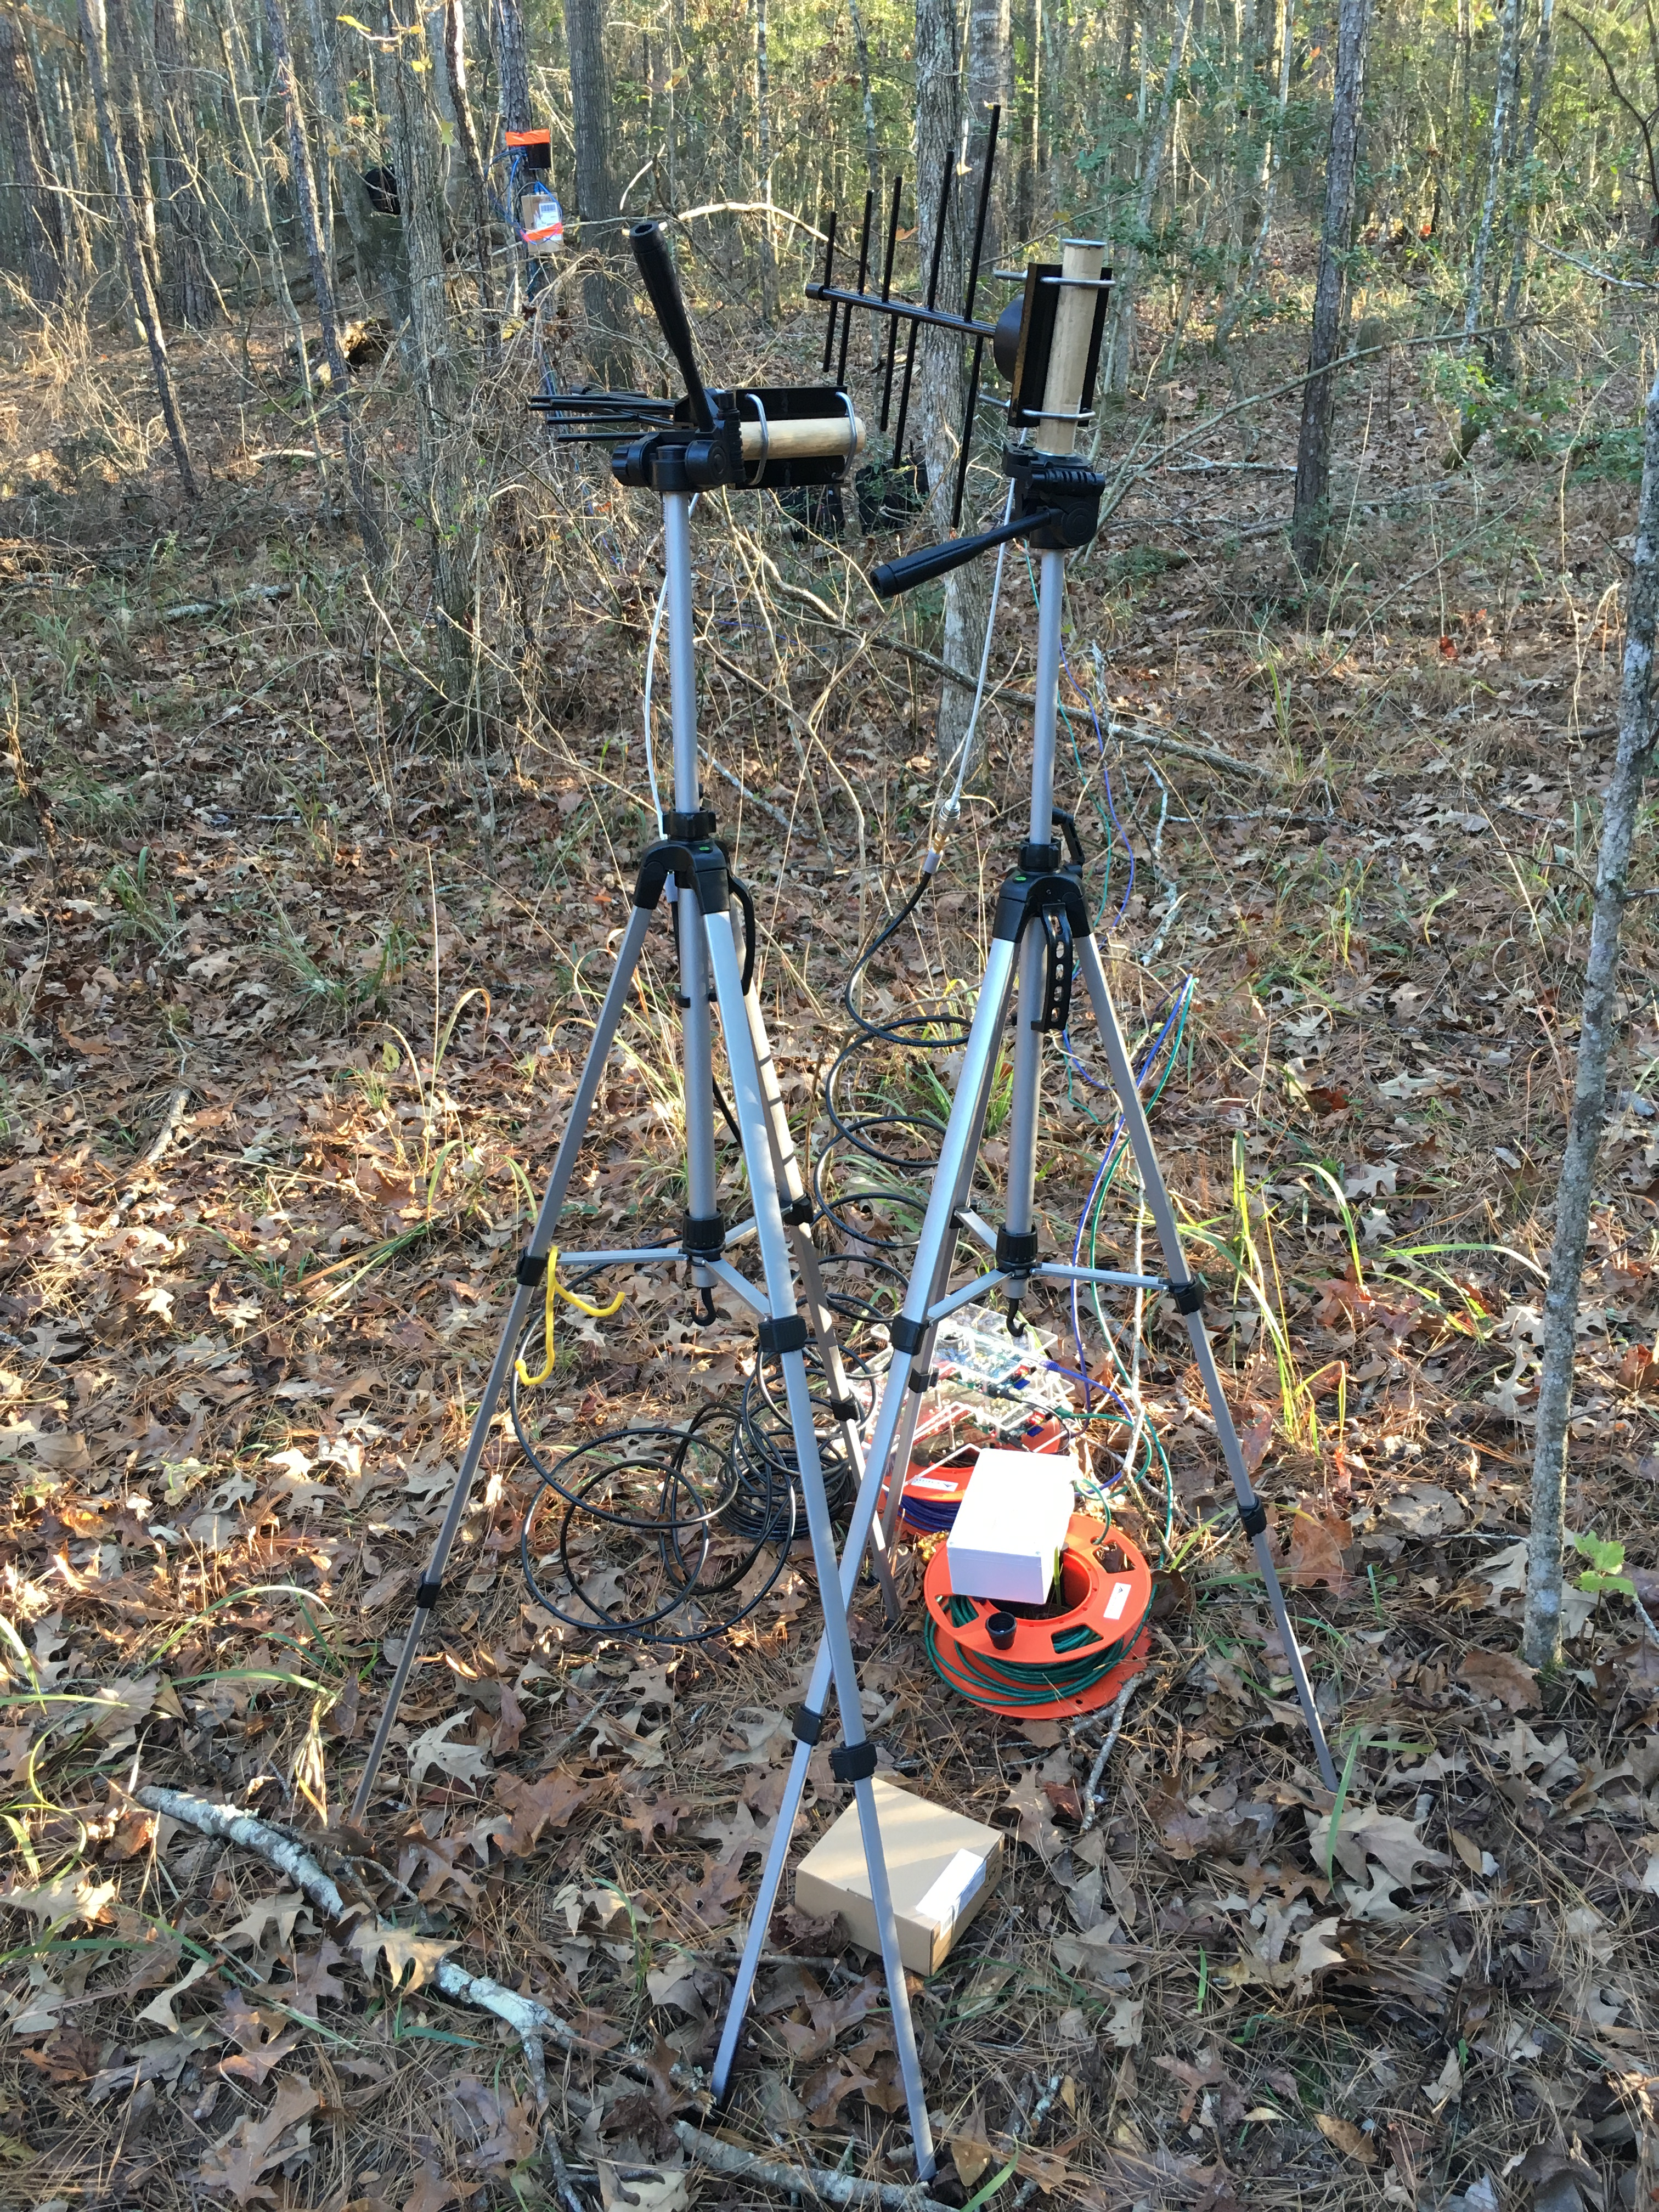
\includegraphics[width=1.0\linewidth]{figs/meas/antenna_horiz_vert_polarization}
\caption{Static \ac{STA} for outdoor tests.}
\label{fig_sta_outdoor_tripod}
\end{minipage}
\end{figure}

\pagebreak

	Two environments were targeted for our measurement campaign: an enterprise indoor environment and a heavily wooded outdoor location.
	We wished to investigate how well outdoor \ac{TVWS} systems performed penetrating trees in a last-mile networks and we wanted to test the superior \ac{NLoS} performance of \ac{TVWS} frequencies.
	Furthermore, we are not aware of any published results for rural \ac{MU-MIMO} systems using anything but elevated \ac{LoS} paths \cite{collings2012ngara}.

\textbf{Indoor Environment.}
	Figure~\ref{fig_mobile_indoor_location} shows the topology of the test network within Duncan Hall, a common classroom and office area at Rice University.
	The 8x8 array was deployed within one room (AP) and six client nodes (STA) are distributed around hallways and stairwells, between 50-100 feet away, at \ac{NLoS} locations indoors.
	The client labeled in black was the mobile client for this test.

\textbf{Outdoor Environment.}
Figure~\ref{fig_array_tree} shows the dense, wooded outdoor environment used, as well as the installation of the Argos-WURC base station at approximately 30 feet above the ground.
Unlike a real base station installation, our test location did not clear the treeline, thus we don't expect superior range performance.
However, it enables us to test a wooded \ac{NLoS} environment whereas additional elevation would make most of the propagation path \ac{LoS}.

We chose the location because it was outside the UHF protection contours of Houston, our home city, as shown by the dropped pin in the coverage map in Figure~\ref{fig_mobile_outdoor_location}.
This figure was obtained from Google's Spectrum Database, and shows unlicensed \ac{TVWS} channels available for operation in green.

Finally, due to our inability to elevate our base station above the 60-foot treeline at our chosen location, our range through the dense forest environment was limited to approximately 600 feet, however \ac{TVWS} connectivity remained robust, while any operation at 2.4~GHz was unreliable beyond a 100 feet.

%% Measurement Technique
\subsection{Multi-user Achievable Rate with Increasing S-T Interval}
\label{sec:uhf_outdoor_results}

 In this section, we investigate the downlink zero-forcing throughput degradation as a function of the S-T interval in indoor and outdoor environments with both nodal and environmental mobility.

 Our evaluation methodology in this section relies on the assumption of channel reciprocity, since it was not yet possible to apply reciprocity calibration to our system when measurements were taken.

 We first record a series of \textit{uplink} channel traces of an 8x4 \ac{MU-MIMO} system with 4 single-radio \acp{STA} using the platform described in Section~\ref{sec_wurc_8x8} with the mobile channel sounding framework presented in Section~\ref{sec_mobile_chan_est}.
 This system is used to record multi-user \ac{CSI} over the course of a minute at regular sampling intervals of 2.5 or 5~ms, timescales chose to balance system performance and memory size of recorded data with the time resolution needed to capture channel dynamics.

 We then assume that the variation in our channel traces is only caused by changes in the physical MIMO channel rather than the radio hardware and use the empirical capacity of the uplink channel in place of the downlink.
 In \cite{guillaud2013reciprocity}, the authors demonstrated channel reciprocity using the same transceivers, and in \cite{shepard2012argos} we demonstrated MIMO reciprocity calibration that we have repeated with our hardware from Section~\ref{sec_wurc_8x8}.
 When accurate reciprocity calibration is performed and interference is identical, the channel in one direction is the same as the other direction.

 Each of six different trials was performed either in a: \emph{(i)} indoor office building environment with non-line-of-sight propagation less than 50~m distance through a wall and a hallway; or \emph{(ii)} the outdoor heavily forested environment shown in Figure~\ref{fig_array_tree} with non-line-of-sight propagation up to 200~m directly through multiple trees and underbrush.
	The tested environments were \textit{static}, with no intentional mobility, \textit{environmental motion}, with pedestrians walking around the fixed \acp{STA}, or \textit{mobile}, with one (indoor) or two (outdoor) \acp{STA} being physically carried by a pedestrian.
		
\begin{figure}[p] % Channel Capacity Loss - Indoor
\centering
\includegraphics[width=1\linewidth]{./figs/protocol/indoor_rate_loss}
\caption{NLOS Indoor hallway 8x4 UHF-band. Colors correspond to STA.}
\label{fig:indoorRateLoss}
\end{figure}

\begin{figure}[p] % Channel Capacity Loss - Outdoor
\centering
\includegraphics[width=1\linewidth]{./figs/protocol/outdoor_rate_loss}
\caption{NLOS Outdoor forest 8x4 UHF-band. Colors correspond to STA.}
\label{fig:outdoorRateLoss}
\end{figure}


	We compare the loss of achievable per-user throughput in Figs.~\ref{fig:indoorRateLoss} and \ref{fig:outdoorRateLoss} as a function of the S-T interval.
 The zero-forcing achievable rate is the percent difference between the rate with fresh \ac{CSIT} and the estimated rate using delayed \ac{CSIT}.

\subsubsection{Effect of Mobility on Achievable Rate}

	We first compare the $8\times4$ zero-forcing results for the various \acp{STA} in Fig.~\ref{fig:indoorRateLoss}.
	When \acp{STA} are static, in Fig.~\ref{fig:indoorRateLoss}a and Fig.~\ref{fig:indoorRateLoss}b, we observe that there is minimal loss of beamforming performance as the S-T interval grows.  While we would expect that little to no change in \ac{CSIT} would occur in the largely static environment in Fig.~\ref{fig:indoorRateLoss}a, an unexpected finding is that environmental mobility, even in the non-line-of-sight environment with pedestrians walking within the same hallway, Fig.~\ref{fig:indoorRateLoss}b, had no significant effect on the averaged beamformed rate.
	Inspecting channel traces, we observe dips in beamforming performance as pedestrians walked by \acp{STA}, but such disruptions were small, momentary and had little effect on the average rate, returning to high rate after the pedestrian had passed.
	Even at 1 second S-T intervals, the system resounds rapidly enough that minimal disruption to the \acp{STA} average capacity is observed.
	
	On the other hand, when the \ac{STA} itself becomes mobile, in Fig.~\ref{fig:indoorRateLoss}c, achievable capacity for the mobile \ac{STA} dropped quickly after an S-T interval of approximately 20~ms.
	This still represents a timescale of tens of packets for a mobile \ac{STA}, indicating that when sufficient uplink traffic is available, an opportunistic sounding \ac{AP} would provide per-user beamforming performance within 15\% of ideal to \textit{mobile} nodes even with S-T interval on the order of a 20~ms. Even under environmental mobility, 15\% of ideal beamforming performance would be achieved with a S-T interval on the order of a second.

\subsubsection{Effect of Environment on Achievable Rate}

	We now repeat the same measurements with the same equipment in the outdoor forest environment in Fig.~\ref{fig:outdoorRateLoss}.
	We chose to perform channel sounding experiments in a heavily forested environment since one of the potential applications of 802.11af \ac{MU-MIMO} networks is to provide last-mile connectivity for residential networks in locations where line-of-sight channels are not available for 802.11ac equipment, which also has severe problems propagating through trees \cite{durgin1998measurements}.
	Parallel 2.4 GHz \ac{MU-MIMO} measurements were attempted at this forested location, yet the signal could barely propagate more than 15~m in the environment and the results were abandoned.
	%\rgnote{The above is anecdotal, but I think it also provides some motivation as to why we're even doing this in the first place--this environment is very hostile to RF propagation and our system performs almost exactly the same as in the indoor environment.}
	
	Our results for the forested environment are similar to the indoor environment: as the S-T interval increases, the average supported capacity of the outdoor \ac{ZFBF} system decreases slowly for the static \acp{STA} and much more rapidly for the mobile \acp{STA}.
	A noticeable difference is that the S-T interval break point for the outdoor mobile nodes appears at approximately 50~ms while in the indoor tests it appears around 20~ms.
	This would be consistent with the outdoor environment that, while also non-line-of-sight, has fewer multi-path reflectors and thus exhibits less channel variation as the \acp{STA} move.


\textbf{\ac{ZFBF} Rate Calculation.}
 Let $P_{jk}$ represent the signal power of spatial stream $j$ received at \ac{STA} $k$.
 If we let $w_{km} \in \mathbf{W}$ be the transmission precoding weight coefficients from \ac{AP} antenna $m$ to \ac{STA} $k$, and $h_{mk} \in \mathbf{H}$ be the corresponding instantaneous \ac{MIMO} 
%\eknote{comically, MIMO gets defined on page 5. a bit of acryonym overload. try to reduce the use of the ac command. too much overall}
channel coefficients at the moment of transmission, we can calculate the empirical transmission \ac{SINR} at \ac{STA} $k$ as the following:
\begin{align}
\text{SINR}_k &= \frac{P_{kk}}{N_k + \sum_{j,j\neq k}P_{jk}} \\
              &= \frac{|\sum_{m=1}^{M}h_{km}w_{mk}|^2}{N_k + \sum_{j,j\neq k} |\sum_{m=1}^{M}h_{km}w_{mj}|^2}. \label{eq_zfbf_capacity}
\end{align}
 Using the well-known Shannon-Hartley theorem, we calculate the empirical achievable rate of the beamformed channel as $R_k = \log{}_2(1+\text{SINR}_k)$.

We find that based on measured beamforming capacity, up to 1 second of S-T interval is allowable to achieve within 15\% of ideal per-user beamforming capacity to fixed \acp{STA}, or 20~ms of S-T interval to achieve within 20\% of ideal beamforming capacity with mobile \acp{STA} in an $8\times4$ zero-forcing system.


\begin{figure}[t] % Sum Channel Capacity Loss
\centering
\includegraphics[width=1\linewidth]{./figs/protocol/sum_rate_loss_w_pow_alloc}
\caption{\ac{NLoS} 8x4 UHF-band sum-rate.}
\label{fig_power_allocation}
%\vspace{-5mm}
\end{figure}

\subsubsection{Effect of Power Allocation}
\label{sec_mobile_sum_rate}

	There are several ways to allocate power when calculating beamforming weights that trade system sum-rate capacity again user fairness.
	Two versions of interest for comparison are waterfilling power allocation, where the majority of the power is allocated to the user with the best channel in order to maximize the sum-rate of the transmission, and equal power allocation, which, as the name suggests, equally allocates transmit power across the \ac{ZFBF} spatial streams without considering their channel quality \cite{spencer2004zero}.
	The performance of alternative power allocation strategies should be predicted by these two characteristic schemes.
	
	We sum the individual results obtained in Figs.~\ref{fig:indoorRateLoss} and \ref{fig:outdoorRateLoss} in Fig.~\ref{fig_power_allocation}, to find that the sum-rate rate loss with increasing S-T interval is somewhat eased when considering the sum network throughput.
	This will be used to simulate opportunistic sounding in Section~\ref{sec:protocolSimulation}.
	
	We also compare the sum-rate achievable rate of our system using equal-power \ac{ZFBF} and waterfilling \ac{ZFBF}.
	As expected, equal power allocation is strictly worse in the sum-rate sense, but there is not a particularly large gap between the two approaches in our tested indoor and outdoor scenarios, indicating that our scenario did not have users with extremely disparate channel power, in which case we would expect a large gap between the two approaches.

%\begin{figure}[t] % Sum Channel Capacity Loss
%\centering
%\includegraphics[width=1\linewidth]{./figs/protocol/sum_rate_loss}
%\caption{\ac{NLoS} 8x4 UHF-band sum-rate.}
%\label{fig:sumRateLoss}
%\vspace{-5mm}
%\end{figure}

\subsubsection{Limits of a fixed S-T interval.}
\label{sec:static_interval}
		In order to gain a more intuitive understanding of our results, we explore our raw channel traces to evaluate the effectiveness of using a fixed S-T interval to achieve a particular performance level.
	Vendors of fixed wireless 802.11 equipment for outdoor operation are increasingly replacing the 802.11 DCF MAC with \ac{TDMA} alternatives for increased long-range efficiency and QoS \cite{unni2015performance} and it is possible that they could guarantee that opportunistic \ac{CSIT} is available with a given S-T interval based on the scheduled uplink/downlink operation of these 802.11 \acp{MAC}. 

 Fig.~\ref{fig:capacity_100ms} depicts two seconds of the empirical achievable rate of the indoor 8x4 \ac{ZFBF} system in order to demonstrate the problem of using fixed resounding intervals.
 The achievable rate of three \acp{STA} are shown in different colors; the solid line is the oracle \ac{ZFBF} rate and the dotted line is the achievable \ac{ZFBF} rate assuming a fixed 100~ms re-sounding interval.
 As expected, the mobile \ac{STA}~1 in blue, which is carried at pedestrian speed within the hallway, demonstrates rapidly changing \ac{CSI} that cannot be tracked accurately by this large fixed sounding interval.
 At each re-sounding point, the periodic system matches the oracle capacity, and then rapidly degrades to approximately 20\% of optimal.
 As the mobile \ac{STA}~1 physically moves by a static \ac{STA}~2 (red, 27 seconds), it perturbs its relatively static wireless channel resulting in severe capacity loss.
 
	Such an event is difficult to predict and could result in outages or large capacity loss unless identified and corrected.
	Based on our observations, a fixed S-T interval would either result in either unnecessary sounding or excessive capacity loss due to stale \ac{CSIT} since channels can change mobility state rapidly.

 We therefore find that an opportunistic sounding policy should have an adaptive component that adjusts the maximum tolerable S-T interval based on current channel conditions and the mobility state of the \ac{STA}.

\begin{figure}[th] % Indoor Capacity Plot with 100ms Resounding
\centering
\includegraphics[width=1\linewidth]{./figs/protocol/indoor_clientmobility_100ms_in}
\caption{8x4 zero-forcing achievable rate, indoor with one mobile \ac{STA} (blue).}
\label{fig:capacity_100ms}
\vspace{-3mm}
\end{figure}

\iftoggle{isready} {

	% Reciprocity calibration for the WURC 8x4 system.
	\subsection{Reciprocity Calibration}
	\label{sec_wurc_reciprocity_cal}

		\rgnote{clean this section or remove it...}

		A necessary technology for scalable \ac{MU-MIMO} is 

	Leveraging the Argos architecture, described in \S\ref{sec:argos}, we implemented and characterized implicit calibration on its Argos-WURC hardware platform. %reciprocal 
	The calibration procedure is implemented in real-time in the node's FPGA fabric, enabling each antenna to send a pilot while all other antennas listen and calculate the channel, with an overhead of just 10 $\mu$s per antenna.
	As long as the radios stay tuned to the same channel, and the temperature does not fluctuate drastically, the calibration is stable indefinitely.
	The instantaneous error of 10,000 measurements across 3 hours is shown in Figure~\ref{fig:calibration_err_time}, and we have verified it is stable for over 12 hours.

		The calibration is very accurate even using just 1 estimation, (a) and (b), and can be much more accurate with more estimations, (c) and (d).
		The calibration is stable, indicating it only needs to be done once at initialization and remains accurate indefinitely. 
		
		Our calibration procedure is highly accurate, as shown in Figure~\ref{fig:calibration_err_cdf} (a) and (b), with an average magnitude error of 0.14\% and an average phase error of 0.43 degrees across three hours when using only a single estimation to calculate the calibration coefficients.
		This error can be further reduced by using multiple calibration estimations, e.g., with 8 estimations this magnitude and phase error is further reduced to 0.048\% and 0.14 degrees, respectively, as depicted in Figure~\ref{fig:calibration_err_cdf} (c) and (d).
		Based on the work in~\cite{lou2013comparison}, implicit calibration within 1.2\% magnitude and 0.5 degrees phase error does not negatively impact the capacity of a zero-forcing \ac{MU-MIMO} wireless system, specifications which our calibration system significantly exceeds. 



	\begin{figure*}[p]
		\centering
		%\captionsetup{justification=centering}
		\subfigure[\small \it Magnitude error.]{ \includegraphics[width=0.45\linewidth]{figs/meas/calibration_mag_err_time}} \hspace{0mm}
		\subfigure[\small \it Phase error.]{\hspace{0mm} \includegraphics[width=0.45\linewidth]{figs/meas/calibration_ang_err_time} \hspace{0mm}}
		\caption{\it Implicit calibration error over 3 hours with no averaging.}
		\label{fig_calibration_err_time}
	\end{figure*}

	\begin{figure*}[p]
		\centering
		%\captionsetup{justification=centering}
		\subfigure[\small \it Magnitude error using 1 estimation.]{ \includegraphics[width=0.45\linewidth]{figs/meas/calibration_mag_err_cdf}} \hspace{0mm}
		\subfigure[\small \it Phase error using 1 estimation.]{\hspace{0mm} \includegraphics[width=0.45\linewidth]{figs/meas/calibration_ang_err_cdf} \hspace{0mm}}
		\subfigure[\small \it Magnitude error using 8 estimations.]{ \includegraphics[width=0.45\linewidth]{figs/meas/calibration_mag_err_cdf_avg}} \hspace{0mm}
		\subfigure[\small \it Phase error using 8 estimations.]{\hspace{0mm} \includegraphics[width=0.45\linewidth]{figs/meas/calibration_ang_err_cdf_avg} \hspace{0mm}}
		\caption{\it CDF of implicit calibration error over 3 hours with and without averaging.}
		\label{fig_calibration_err_cdf}
	\end{figure*}
	
}


%% Mobile UHF-band Measurements Conclusions
%\subsection{Discussion and Conclusion}
%\label{sec_mobile_measurements_conclusion}

	
 